%!TEX TS-program = ../make.zsh

\subsection{Hole-Ice as Cylinder-Shaped Ice Areas With Differing Photon-Propagation Properties}

In the \icecube simulation framework, photon propagation simulation takes several dependencies into account: The photon absorption length and the photon scattering length may depend on the photon's wave length. Absorption and scattering length may also depend on the photon's $z$-coordinate as the South-Polar ice consists of several \textit{ice layers}. These ice layers may also be tilted. Furthermore, the absorption length may depend on the photon's direction of motion, which is called \textit{absorption anisotropy}.

This study adds another ice feature to the simulation: Hole ice may be modeled by adding cylinder-shaped areas within the surrounding bulk ice where the propagation properties, that is to say the photon's absorption length and scattering length, differ from the propagation properties of the bulk ice.

Figure \ref{fig:aiw2Thah} illustrates such a scenario for one single photon: The photon's trajectory starts in the bulk ice. The photon enters the hole-ice cylinder where the scattering length is shorter as in the bulk ice. Hence the photon scatters more frequently within the cylinder. When the photon leaves the hole-ice cylinder the propagation properties of the bulk ice take effect again, resulting in the photon scattering less frequently after leaving the cylinder.

\begin{figure}[htb]
  \centering
  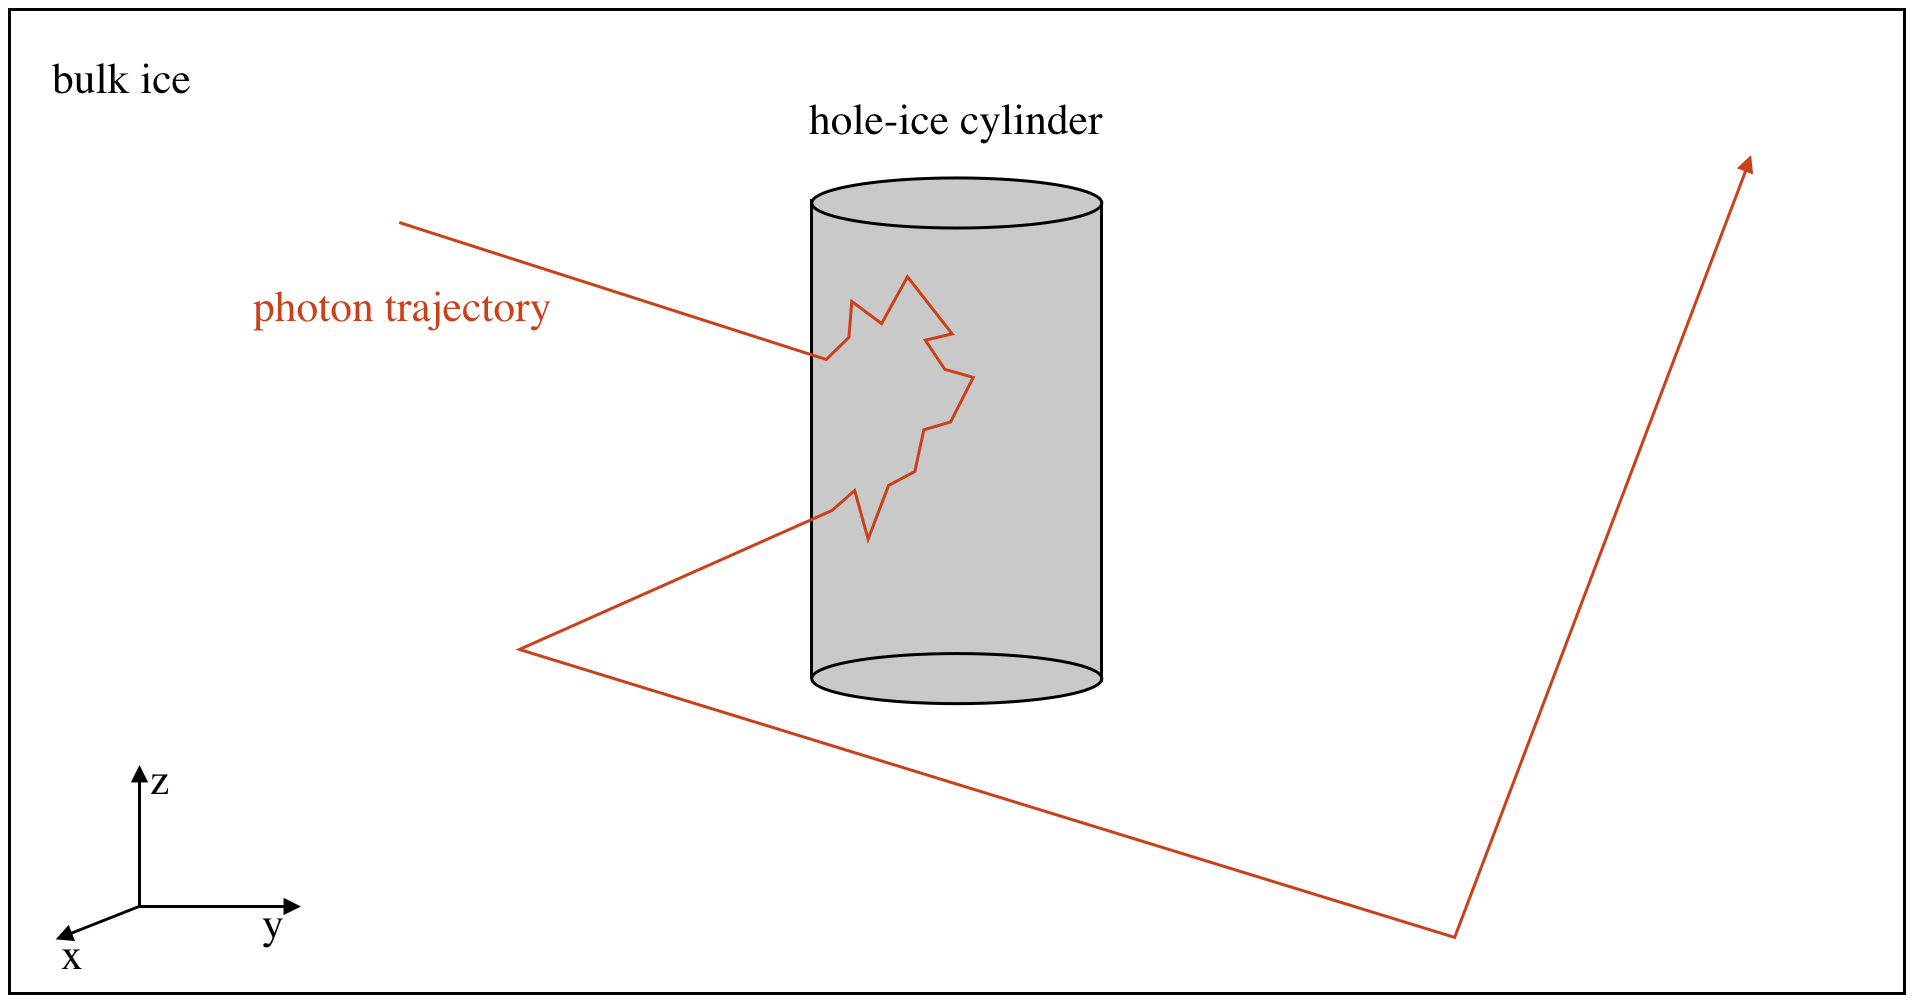
\includegraphics[width=0.6\textwidth]{img/hole-ice-as-cylinder-shaped-areas}
  \caption{Schematic diagram of a propagating photon. The photon enters a hole-ice cylinder with a scattering length different from the outside ice. When leaving the cylinder the photon assumes the scattering length of the outside ice again.}
  \label{fig:aiw2Thah}
\end{figure}

In this study, cylinders are always defined along the $z$-axis. Also, the scattering angle is assumed to behave the same within the hole-ice cylinders as in the bulk ice.
% because there has been no indication provided by experimental data or theoretical ice models on how the scattering angle should behave differently within the hole ice.

